\chapter{ Cybersecurity }

\section{Introduzione alla sicurezza informatica}
Il rapporto interno/interagenzia NIST NISTIR 7298 (Glossario di informazioni chiave
Termini di sicurezza, maggio 2013) definisce il termine sicurezza informatica  come segue:

\begin{center}
    \textit{Misure e controlli che garantiscono riservatezza, integrità,
    e disponibilità delle risorse del sistema informativo inclusi hardware, software, firmware,
    e le informazioni che vengono elaborate, archiviate e comunicate.}
\end{center}


Questa definizione introduce tre obiettivi chiave che sono al centro della cybersecurity:

\begin{itemize}
    \item \textbf{Confidentiality} (Riservatezza):  conservazione delle restrizioni autorizzate all'accesso alle informazioni e divulgazione, compresi i mezzi per proteggere la privacy personale e le proprie informazione. Una perdita di riservatezza è la divulgazione non autorizzata di informazioni. Questo termine copre due concetti correlati:
    \begin{itemize}
        \item  \textbf{Data Confidentiality} : garantisce che le informazioni private o riservate non siano disponibili o divulgate a soggetti non autorizzati.
        \item \textbf{Privacy}: assicura che le persone controllino o influenzino le informazioni
        ad essi relativi, esse possono essere raccolte e conservate, inoltre si definisce da chi e a chi possono essere divulgate.
    \end{itemize}
    \item \textbf{Integrity} (Integrità): prevenire la modifica o la distruzione impropria delle informazioni, compresa la garanzia del non ripudio e dell'autenticità delle informazioni. Una perdita di l'integrità è la modifica o la distruzione non autorizzata di informazioni. Questo termine copre due concetti correlati:
    \begin{itemize}
        \item \textbf{Data integrity}:  garantisce che le informazioni e i programmi vengano modificati solo in modo determinato e autorizzato.
        \item \textbf{System integrity}: assicura che un sistema svolga la sua funzione prevista in modo inalterato, libero da intenzionali o involontarie manipolazioni non autorizzate del sistema.
    \end{itemize}
    \item \textbf{Availability}(Disponibilità): garantisce un accesso tempestivo e affidabile nell'utilizzo delle informazioni. Una perdita di disponibilità è l'interruzione dell'accesso o dell'uso di informazioni o un sistema informativo.
\end{itemize} 

\noindent
Questi tre concetti formano quella che viene spesso definita la triade della CIA. I tre
concetti incarnano gli obiettivi di sicurezza fondamentali sia per i dati che per le informazioni
e servizi informatici. Ad esempio, lo standard FIPS 199 del NIST (Standards for Security
Categorization of Federal Information and Information Systems , febbraio 2004) elenca la riservatezza, integrità e disponibilità come i tre obiettivi di sicurezza per le informazioni e
per i sistemi informativi.
\begin{figure}[H]
	\centering
    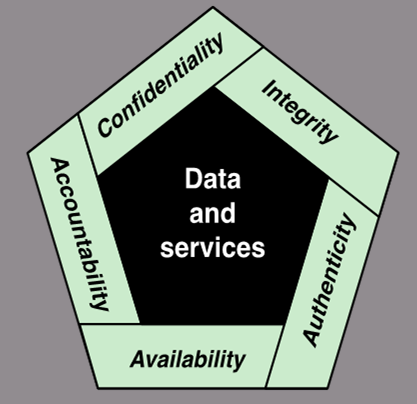
\includegraphics[width=7cm, keepaspectratio]{Bistarelli/img/cap_1/cia.png}
	\caption{Requisiti essenziali in Cybersecurity.}\label{fig:cia}
\end{figure}

Sebbene l'uso della triade della CIA per definire gli obiettivi di sicurezza sia ben consolidato,
alcuni nel campo della sicurezza ritengono che siano necessari concetti aggiuntivi da presentare
un quadro completo. Due dei più comunemente citati sono i seguenti:
\begin{itemize}
    \item \textbf{Authenticity} (Autenticità): la proprietà di essere genuini e di poter essere verificati e di essere trusted. Fiducia nella validità di una trasmissione di un messaggio o di un messaggio originatore. Ciò significa verificare che gli utenti siano chi dicono di essere e che ogni input che arriva al sistema proviene da una fonte attendibile.
    \item \textbf{Accountability}(Rendicontabilità): è la capacità di un sistema di identificare un singolo utente, di determinarne le azioni e il comportamento all'interno del sistema stesso. La rendicontabilità è un aspetto del controllo di accesso e si basa sulla concezione che gli individui siano responsabili delle loro azioni all'interno del sistema. Questo supporta il non ripudio, deterrenza, isolamento dei guasti, rilevamento e prevenzione delle intrusioni, il recupero post-azione in concomitanza con l'azione legale . Poiché i sistemi veramente sicuri non sono ancora un obiettivo realizzabile, dobbiamo essere in grado di tracciare una violazione della sicurezza al/ai responsabile/i. I sistemi devono tenere traccia delle loro attività per consentire successive analisi forensi per rintracciare violazioni della sicurezza o per aiutare nelle controversie sulle transazioni.
\end{itemize}
Si noti che FIPS 199 include l'autenticità sotto integrità.
\\
La sicurezza informatica è allo stesso tempo affascinante e complessa, alcuni dei motivi sono:
\begin{enumerate}
    \item \textit{La sicurezza informatica non è così semplice come potrebbe sembrare a un principiante}. I requisiti sembrano essere semplici,in effetti, la maggior parte dei requisiti principali per i servizi di sicurezza possono essere definiti con etichette formate autoesplicative formate da una sola parola: riservatezza, autenticazione, non ripudio e integrità. Ma i meccanismi utilizzati per soddisfare tali requisiti possono essere piuttosto complessi, e capirli può portare a un ragionamento piuttosto sottile.
    \item \textit{Nello sviluppo di un particolare meccanismo di sicurezza o algoritmo, bisogna sempre considerare potenziali attacchi a tali funzionalità di sicurezza.} In molti casi gli attacchi di successo sono progettati guardando un problema in un modo completamente differente, dunque sfruttando una debolezza inaspettata del meccanismo.
    \item \textit{A causa del punto 2 , le procedure usate per fornire dei servizi particolari sono spesso controintuitive.} Tipicamente, un meccanismo di sicurezza è complesso e non è ovvio dalle dichiarazioni di una particolare esigenza che tali misure elaborate sono necessarie. Solo quando si prendono in considerazione i vari aspetti della minaccia si elaborano i meccanismi di sicurezza hanno un senso.
    \item \textit{I meccanismi di sicurezza in genere coinvolgono più di un particolare algoritmo o
    protocollo.}Richiedono inoltre che i partecipanti siano in possesso di un'informazione segreta (ad es. una chiave di crittografia), che sollevano domande sulla creazione, distribuzione e protezione di tali informazioni segrete. Potrebbe esserci anche una dipendenza sui protocolli di comunicazione il cui comportamento può complicare il compito di sviluppare il meccanismo di sicurezza. Ad esempio, se il corretto funzionamento del meccanismo di sicurezza richiede la definizione di limiti di tempo per il tempo di transito di un messaggio dal mittente al destinatario, allora qualsiasi protocollo o rete che introduce variabili e/o ritardi imprevedibili può rendere tali termini privi di significato.
    \item \textit{ La sicurezza informatica è essenzialmente una battaglia di ingegni tra un perpetratore che prova a  trovare buchi e il progettista o l'amministratore che tenta di chiuderli.} Il grande vantaggio che l'attaccante ha è che lei o lui ha solo bisogno di trovare una singola vulnerabilità, mentre il progettista deve trovare e eliminare tutte le vulnerabilità per ottenere una sicurezza perfetta.
    \item \textit{La sicurezza è ancora troppo spesso un'"aggiunta" (surplus) per essere incorporata in un sistema dopo che il progetto è completo, piuttosto che essere parte integrante del processo di progettazione.}
    \item \textit{La sicurezza richiede un monitoraggio regolare, anche costante, e questo è difficile nei tempi attuali.}
    \item \textit{C'è una naturale tendenza da parte di utenti e gestori di sistema a percepire pochi vantaggi nell'investimento sulla sicurezza fino a quando non si verifica un problema.}
    \item \textit{ Molti utenti e persino gli amministratori della sicurezza vedono una sicurezza forte come un ostacolo al funzionamento o all'uso efficiente di un sistema informativo o di un'informazione.}
\end{enumerate}

\subsection{Terminologie}
La maggior parte delle terminologie sono riportate nel Capitolo \ref{ch:terminologie} degli appunti Prof. Santini, di seguito riporto alcuni termini non citati in precedenza.

\subsubsection{Risorsa di sistema (Asset)}
Una applicazione maggiore, un sistema di supporto generale, un programma ad alto impatto,un impianto fisico, un sistema mission-critical, personale, apparecchiature o un gruppo di sistemi logicamente correlati.  

\subsubsection{Minaccia}
Qualsiasi circostanza o evento che potrebbe avere un impatto negativo sulle operazioni organizzative (inclusi missione, funzioni, immagine o reputazione), risorse organizzative, individui, altre organizzazioni o la Nazione stessa attraverso un sistema informativo tramite accesso, distruzione, divulgazione, modifica non autorizzati delle informazioni , e/o negazione del servizio.

\subsubsection{Contromisure}
Dispositivo o tecniche che hanno come obiettivo la compromissione dell'efficacia operativa di attività indesiderate o contraddittorie, o la prevenzione di spionaggio, sabotaggio, furto o accesso o utilizzo non autorizzato di informazioni sensibili o di sistemi informativi.

\subsubsection{Rischio}
Una misura del grado in cui un'entità è minacciata da una potenziale circostanza o evento, e tipicamente una funzione di stima:
\begin{enumerate}
    \item  degli impatti negativi che si verificherebbero se la circostanza o l'evento si verificassero
    \item  della probabilità che si verifichi.
\end{enumerate}

\begin{figure}[H]
	\centering
    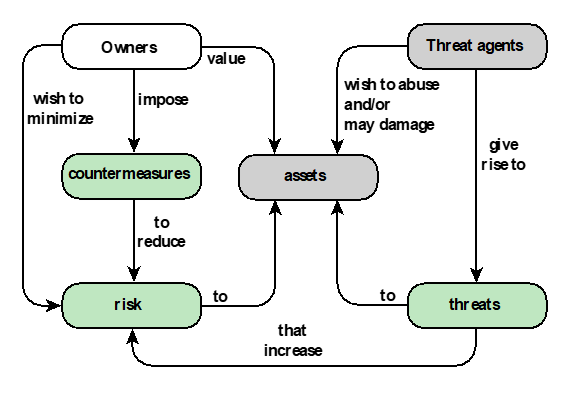
\includegraphics[width=11cm, keepaspectratio]{Bistarelli/img/cap_1/relazione_concetti_sicurezza.png}
	\caption{Concetti di sicurezza e le loro relazioni.}\label{fig:relazioni_concetti_sec}
\end{figure}

\subsection{Asset di un sistema informatico}
Gli asset di un sistema informatico possono essere suddivisi come di seguito:
\begin{itemize}
    \item \textbf{Hardware}: compresi i sistemi informatici e altri trattamenti di dati, archiviazione dei dati,e dispositivi di comunicazione dati;
    \item \textbf{Software}: include il sistema operativo, le utilità di sistema e le applicazioni;
    \item \textbf{Data}: inclusi file e database, nonché dati relativi alla sicurezza, ad esempio file di password. 
    \item \textbf{Strutture e reti di comunicazione}: rete locale e geografica collegamenti di comunicazione, bridge, router e così via.
\end{itemize}

\subsection{Vulnerabilità, minacce e attacchi}
Nel contesto della sicurezza, la nostra preoccupazione riguarda le vulnerabilità delle risorse del sistema. [NRC02] elenca le seguenti categorie generali di vulnerabilità di un sistema informatico o di una risorsa di rete:
\begin{itemize}
    \item Il sistema può essere danneggiato (\textbf{corrupted}), quindi fa la cosa sbagliata o dà risposte sbagliate. Ad esempio, i valori dei dati memorizzati possono differire da quello che dovrebbero essere perché sono stati modificati in modo improprio.
    \item Il sistema avere delle perdite (\textbf{be leaky}). Ad esempio, qualcuno che non dovrebbe avere accesso ad alcune o a tutte le informazioni disponibili attraverso la rete ottengono tale accesso.
    \item Il sistema può diventare non disponibile (\textbf{unavailable}) o molto lento. Cioè, usando il sistema o la rete diventa impossibile o impraticabile.
\end{itemize}
Questi tre tipi generali di vulnerabilità corrispondono ai concetti di integrità, riservatezza e disponibilità, enumerati in precedenza. Una \textbf{minaccia} rappresenta un potenziale danno alla sicurezza di una risorsa. Un \textbf{attacco} è una minaccia che viene eseguita (azione di minaccia) e, in caso di successo, comporta una violazione indesiderata della sicurezza o a una conseguenza della minaccia. L'agente che effettua l'attacco viene definito \textbf{attaccante} o \textbf{agente di minaccia}. Possiamo distinguere gli attacchi in due tipi:
\begin{itemize}
    \item \textbf{Attacco attivo}: un tentativo di alterare le risorse del sistema o di influenzare il funzionamento.
    \item \textbf{Attacco passivo}: un tentativo di imparare o di fare use delle informazioni da un sistema che non influenza le risorse di quest'ultimo.
\end{itemize}

\noindent
Possiamo classificare gli attacchi in base all'origine di questi:
\begin{itemize}
    \item \textbf{Attacco interno}: iniziato da un entità interna al perimetro di sicurezza ( un "insider"). L'insider è autorizzato all'accesso alle risorse del sistema ma le usa in un modo non approvato da coloro che ne garantiscono l'accesso.  
    \item \textbf{Attacco esterno}: iniziato fuori dal perimetro, da un utente non autorizzato o illegittimo del sistema (un "outsider"). Su Internet, potenziale aggressori esterni variano dai dilettanti "burloni" a criminali organizzati, internazionali terroristi e governi ostili.
\end{itemize}

Infine, una contromisura è qualsiasi mezzo adottato per affrontare un attacco alla sicurezza. Idealmente, una contromisura può essere escogitata per prevenire un particolare tipo di attacco dall'avere successo. Quando la prevenzione non è possibile, o in alcuni casi fallisce, l'obiettivo è rilevare l'attacco e poi riprendersi dagli effetti . Una contromisura stessa può introdurre nuove vulnerabilità. In ogni caso, vulnerabilità residue
possono rimanere dopo l'imposizione di contromisure. Tali vulnerabilità possono essere sfruttato da attaccanti che rappresentano un livello di rischio residuo per gli asset. I proprietari dell'asset cercheranno di ridurre al minimo tale rischio dati altri vincoli.


\begin{figure}[H]
	\centering
    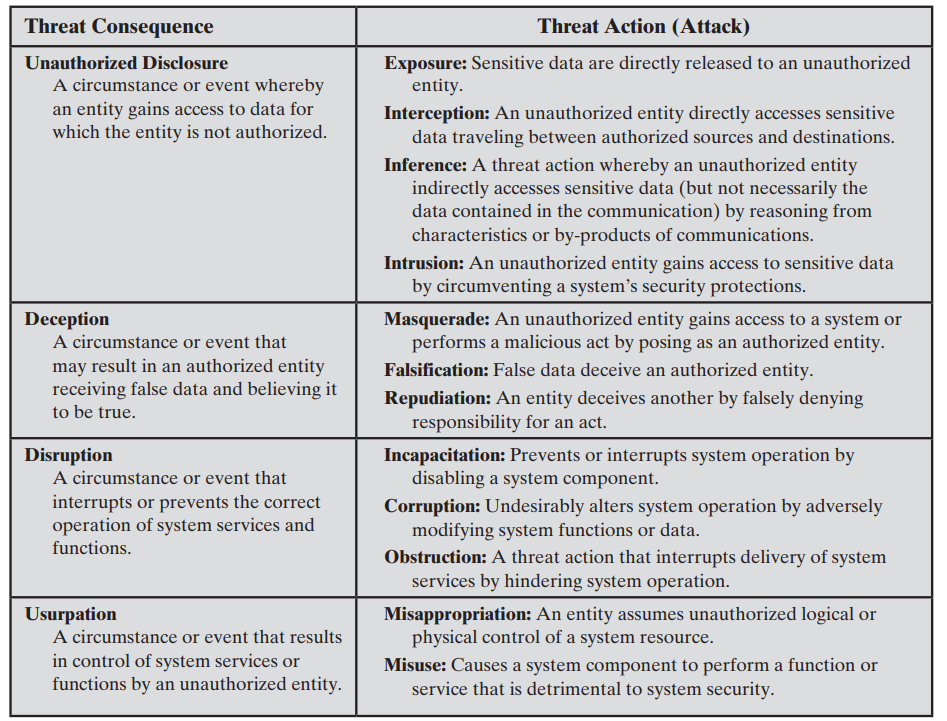
\includegraphics[width=14cm, keepaspectratio]{Bistarelli/img/cap_1/tabella_minacce.png}
	\caption{Conseguenze delle minacce e azioni che le causano }\label{fig:tabella_minacce}
\end{figure}

La tabella \ref{fig:tabella_minacce} basata su RFC 4949, descrive quattro tipi di conseguenze ed elenca i tipi di attacchi che risultano in ciascuna conseguenza. 

La divulgazione non autorizzata (Unauthorized disclosure) è una minaccia alla riservatezza. I seguenti tipi di attacchi possono portare a queste conseguenze

\begin{itemize}
    \item \textbf{Esposizione}: quando un insider rilascia intenzionalmente informazioni sensibili a un estraneo, come ad esempio i numeri di carta di credito. Può anche essere il risultato di un errore umano, hardware o software, che si traduce nell'azione da parte di un'entità di avere l'accesso non autorizzato di dati sensibili. Ce ne sono stati numerosi casi di questo, come le università che pubblicano accidentalmente le informazioni confidenziali degli studenti sul Web.
    \item \textbf{Intercettazione}: l'intercettazione è un attacco comune nel contesto delle comunicazioni. Su una rete locale condivisa (LAN), come una LAN wireless o a broadcast Ethernet, qualsiasi dispositivo collegato alla LAN può ricevere una copia dei pacchetti destinati a un altro dispositivo. Su Internet, un determinato hacker può accedere al traffico di posta elettronica e ad altri trasferimenti di dati. Tutte queste situazioni possono portare all'accesso non autorizzato ai dati.
    \item \textbf{Inferenza}: un esempio di inferenza è noto come analisi del traffico, in cui un avversario è in grado di ottenere informazioni osservando l'andamento del traffico una rete, come la quantità di traffico tra particolari coppie di host sulla rete. Un altro esempio è l'inferenza di informazioni dettagliate da un database di un utente che ha solo un accesso limitato, questo è realizzato da query ripetute i cui risultati combinati consentono l'inferenza.
    \item \textbf{Intrusione}: un esempio di intrusione è un avversario che ottiene l'accesso non autorizzato a dati sensibili superando le protezioni di controllo degli accessi del sistema.
\end{itemize}

L'inganno (Deception) è una minaccia per l'integrità del sistema o per l'integrità dei dati. I seguenti tipi di attacchi possono portare a queste conseguenze:
\begin{itemize}
    \item \textbf{Masquerade}: un esempio di masquerade è un tentativo di accesso a un sistema  da parte di un utente non autorizzato spacciandosi per uno autorizzato, questo può succedere se l'utente non autorizzato conosce l'ID di accesso e la password di un altro utente. Un altro esempio è la logica dannosa (malicious logic), come un cavallo di Troia, che appare per eseguire una funzione utile o desiderabile, ma in realtà ottiene l'accesso non autorizzato alle risorse di sistema o induce un utente a eseguire altre logiche dannose.
    \item \textbf{Falsificazione}: si riferisce all'alterazione o sostituzione di dati validi o all'introduzione di dati falsi in un file o database. Ad esempio, uno studente può alterare i suoi voti su un database scolastico.
    \item \textbf{Ripudio}: in questo caso, un utente nega l'invio di dati o nega di ricevere o possedere i dati.
\end{itemize}

L'interruzione (Disruption) è una minaccia alla disponibilità o all'integrità del sistema. I seguenti tipi di attacchi possono portare a queste conseguenze:
\begin{itemize}
    \item \textbf{Incapacità}: questo è un attacco alla disponibilità del sistema. Ciò potrebbe verificarsi come risultato della distruzione fisica o del danneggiamento dell'hardware del sistema. Più tipicamente, un software dannoso, come Trojan, virus o worm, potrebbero operarein modo tale da disabilitare un sistema o alcuni dei suoi servizi.
    \item \textbf{Corruzione}: questo è un attacco all'integrità del sistema. Un Software dannoso in questo contesto potrebbe funzionare in modo tale che le risorse di sistema o i servizi funzionino in modo non intenzionale. Oppure un utente potrebbe ottenere l'accesso non autorizzato a un sistema e modificarne alcune funzioni. Un esempio di quest'ultimo è un posizionamento di una logica backdoor (backdoor logic) nel sistema per fornire il successivo accesso al sistema stesso e alle sue risorse con una procedura diversa da quella abituale.
    \item \textbf{Ostruzione}: un modo per ostacolare il funzionamento del sistema è interferire con le comunicazioni disabilitando i collegamenti di comunicazione o alterando la comunicazione delle informazioni di controllo. Un altro modo è sovraccaricare il sistema mettendo un carico in eccesso sul traffico di una comunicazione o sulle risorse di elaborazione.
\end{itemize}

L'usurpazione (Usurpation) è una minaccia per l'integrità del sistema. I seguenti tipi di attacchi possono portare a queste conseguenze:
\begin{itemize}
    \item \textbf{Appropriazione indebita}: può includere il furto del servizio. Un esempio è un attacco Denial of Service distribuito, quando il software dannoso è installato su degli host da utilizzare come piattaforme per avviare il traffico verso un host di destinazione. In questo caso, il software maligno fa uso non autorizzato delle risorse del processore e del sistema operativo.
    \item \textbf{Uso improprio}: l'uso improprio può verificarsi per mezzo di una malicious logic o di un hacker che ha ottenuto un accesso non autorizzato a un sistema. In entrambi i casi, le funzioni di sicurezza possono essere disabilitate o contrastate.
\end{itemize}

\subsection{Asset e minacce}
Le risorse di un sistema informatico possono essere classificate come hardware, software, dati, linee e reti di comunicazione. In questa sottosezione li descriviamo brevemente e mettendoli in relazione con i concetti di integrità, riservatezza e
disponibilità. 

\begin{figure}[H]
	\centering
    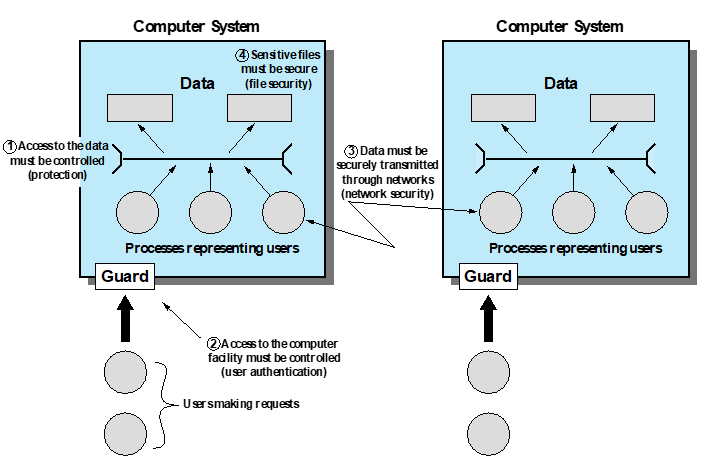
\includegraphics[width=14cm, keepaspectratio]{Bistarelli/img/cap_1/asset_sec.png}
	\caption{ Scopo della sicurezza informatica.}\label{fig:asset_sec}
\end{figure}

\paragraph{Hardware.} Una delle principali minacce per l'hardware  del computer è la minaccia alla disponibilità. L'hardware è il più vulnerabile agli attacchi e il meno suscettibile ai controlli automatizzati. Le minacce includono danni accidentali e deliberati alle apparecchiature così come il furto. La proliferazione di personal computer e workstation e l'uso diffuso delle LAN aumenta il potenziale di perdite in quest'area. Il furto delle unità USB può portare alla perdita di riservatezza. Le misure di sicurezza fisiche e amministrative sono necessarie per far fronte a queste minacce.


\paragraph{Software.} Il software include il sistema operativo, le utilità e l'applicazione programmi. Una delle principali minacce al software è un attacco alla disponibilità. Il Software, in particolare quello applicativo, è spesso facile da eliminare. Il software può anche essere modificato o danneggiato per renderlo inutilizzabile. Un'attenta gestione della configurazione del software, che include il mantenere dei backup della versione più recente, può mantenere una disponibilità alta. Un problema più difficile da affrontare è la modifica del software che si ha in un programma il quale funziona ancora ma che si comporta in modo diverso rispetto a prima,
questa è una minaccia per l'integrità/autenticità. Rientrano in questa categoria i virus informatici e i relativi attacchi. Un ultimo problema è la protezione contro la pirateria del software. Sebbene siano disponibili alcune contromisure, in linea di massima il problema di copie non autorizzate del software non è stata risolta.

\paragraph{Data.}  Un  problema molto più diffuso è la sicurezza dei dati, che coinvolge file e altre forme di dati controllati da individui, gruppi e organizzazioni aziendali.

I problemi di sicurezza relativi ai dati sono ampi e comprendono disponibilità, segretezza e integrità. In caso di disponibilità, la preoccupazione è con la distruzione di file di dati, che può verificarsi accidentalmente o intenzionalmente. 
Una preoccupazione evidente per la segretezza è la lettura non autorizzata di file di dati o database, e quest'area è stata forse oggetto di ulteriori ricerche e sforzi rispetto a qualsiasi altro settore della sicurezza informatica. Una minaccia meno ovvia alla segretezza comporta l'analisi dei dati e si manifesta nell'utilizzo delle cosiddette banche dati statistiche, che forniscono informazioni di sintesi o aggregate. Presumibilmente, l'esistenza delle informazioni aggregate non minacciano la privacy delle persone coinvolte. Tuttavia, con la crescita dell'uso delle banche dati statistiche, c'è un rischio crescente per la divulgazione di informazioni personali. In sostanza, le caratteristiche di un individuo possono essere identificate attraverso un'analisi attenta. Ad esempio, se una tabella registra l'aggregato dei redditi degli intervistati A, B, C e D e un altro registra l'aggregato dei redditi di A, B, C, D ed E, la differenza tra i due aggregati sarebbe il reddito di E. Questo problema è esasperato dal desiderio crescente di combinare set di dati. In molti casi, abbinando diversi set di dati per coerenza tra i diversi livelli di aggregazione è necessario l'accesso alle singole unità. Pertanto, le singole unità, che sono oggetto di problemi di privacy, sono disponibili in varie fasi del trattamento dei set di dati. 
Infine, l'integrità dei dati è una delle principali preoccupazioni nella maggior parte delle installazioni.Le modifiche ai file di dati possono avere conseguenze che vanno da minori a disastrose.

\subsection{Attacchi passivi e attivi}
Gli attacchi alla sicurezza della rete possono essere classificati
come attacchi passivi e attacchi attivi. Un attacco passivo tenta di imparare o fare
uso delle informazioni del sistema, ma non influisce sulle risorse di quest'ultimo. Un attacco attivo tenta di alterare le risorse di sistema o di influenzare il loro funzionamento.

\subsubsection{Attacchi passivi}
Gli \textbf{attacchi passivi} generalmente riguardano l'intercettazione o il monitoraggio di trasmissioni di dati. L'obiettivo dell'attaccante è ottenere le informazioni che vengono trasmesse. Due tipi di attacchi passivi sono il rilascio del contenuto dei messaggi e dell'analisi del traffico.

\paragraph{Rilascio dei contenuti di un messaggio} Il \textbf{rilascio dei contenuti} del messaggio è facilmente comprensibile. Una conversazione telefonica, un messaggio di posta elettronica e un file trasferito possono contenere dati sensibili o informazioni confidenziali. Vorremmo impedire a un avversario di imparare il contenuto di queste trasmissioni.

\paragraph{Analisi del traffico.} Un secondo tipo di attacco passivo, \textbf{l'analisi del traffico}, è più sottile. Supponiamo che noi abbiamo un modo per mascherare il contenuto dei messaggi o altre informazioni del traffico di dati, in modo che gli oppositori, anche se hanno catturato il messaggio, non possono estrarre le informazioni dal messaggio. La tecnica comune per mascherare i contenuti è la crittografia. Anche se disponiamo di una protezione crittografica, un avversario potrebbe comunque essere in grado di osservare lo schema di questi messaggi. L'avversario potrebbe determinare la posizione e l'identità degli host nella comunicazione e potrebbe osservare la frequenza e la lunghezza dei messaggi scambiati. Queste informazioni potrebbero essere utili per indovinare la natura della comunicazione che stava avvenendo.

Gli attacchi passivi sono molto difficili da rilevare perché non coinvolgono alterazione dei dati. In genere, il traffico dei messaggi viene inviato e ricevuto in un modo apparentemente normale e né il mittente né il destinatario sono consapevoli che una terza parte ha letto i messaggi o osservato l'andamento del traffico. Tuttavia, è possibile prevenire il successo di questi attacchi, di solito mediante crittografia. Pertanto, l'enfasi nell'affrontare gli attacchi passivi è sulla prevenzione piuttosto che il rilevamento.

\subsubsection{Attacchi attivi}
Gli attacchi attivi comportano alcune modifiche del flusso di dati o la creazione
di un falso flusso, esso può essere suddiviso in quattro categorie: replay, masquerade, modifica dei messaggi e denial of service.

\paragraph{Replay.} Il replay comporta l'acquisizione passiva di un'unità di dati e la sua successiva ritrasmissione per produrre un effetto non autorizzato.


\paragraph{Masquerade.} Una masquerade ha luogo quando un'entità finge di essere un'entità diversa. Un attacco di questo tipo di solito include una delle altre forme di attacco attivo. Per esempio, le sequenze di autenticazione possono essere catturate e riprodotte dopo che è avvenuta una sequenza di autenticazione valida, abilitando così un'entità autorizzata con pochi privilegi a ottenere privilegi extra impersonando un'entità che dispone di tali privilegi.

\paragraph{Modifica di un messaggio.} La modifica dei messaggi significa semplicemente che una parte di un legittimo messaggio è alterato, o che i messaggi sono ritardati o riordinati, per produrre un effetto non autorizzato. Ad esempio, un messaggio che afferma: "Consenti a John Smith di leggere dati di file riservati" viene modificato per dire "Consenti a Fred Brown di leggere dati di file riservati".

\paragraph{DOS.} La negazione del servizio impedisce o inibisce il normale utilizzo o gestione delle strutture di comunicazione. Questo attacco può avere un obiettivo specifico, per esempio un'entità può sopprimere tutti i messaggi diretti a una particolare destinazione (ad esempio, la sicurezza del servizio di audit). Un'altra forma di rifiuto del servizio è l'interruzione di un'intera rete, o disabilitando la rete o sovraccaricandola di messaggi in modo da degradarne le prestazioni.

Gli attacchi attivi presentano le caratteristiche opposte degli attacchi passivi. Invece gli attacchi passivi sono difficili da rilevare, sono disponibili misure per prevenirli con successo. D'altra parte, è abbastanza difficile prevenire assolutamente gli attacchi attivi, perché per farlo richiederebbe la protezione fisica di tutte le strutture e i percorsi di comunicazione in ogni momento. Invece, l'obiettivo è rilevarli e riprendersi da qualsiasi disservizio o ritardi da essi causati. Poiché il rilevamento ha un effetto deterrente, esso può anche contribuire alla prevenzione.

\subsection{Requisiti di sicurezza} 
Esistono diversi modi per classificare e caratterizzare le contromisure che possono essere utilizzate per ridurre le vulnerabilità e affrontare le minacce alle risorse di sistema. In questa sottosezione, vediamo contromisure in termini di requisiti funzionali, e seguiamo la classificazione definita in FIPS 200. Questo standard enumera 17 aree relative alla sicurezza con riguardo alla protezione della riservatezza, dell'integrità e della disponibilità delle informazioni di sistemi e le informazioni elaborate, archiviate e trasmesse da tali sistemi.
\begin{enumerate}
    \item \textbf{Accesso controllato}: limitare l'accesso al sistema informativo agli utenti autorizzati, ai processi che agiscono per conto degli utenti autorizzati, o ai dispositivi (inclusi altri sistemi informativi) e alle tipologie di transazioni e funzioni che gli utenti autorizzati possono esercitare.
    \item \textbf{Consapevolezza e Formazione}: garantire che i gestori e gli utenti dei sistemi informativi organizzativi siano consapevole dei rischi per la sicurezza associati alle proprie attività e delle leggi, dei regolamenti e delle politiche applicabili relativi alla sicurezza dei sistemi informativi organizzativi e  garantire che il personale sia adeguatamente addestrato a svolgere i compiti e le responsabilità assegnate in materia di sicurezza delle informazioni.
    \item \textbf{Audit e responsabilità}: creare, proteggere e conservare i record di audit del sistema informativo per consentire il monitoraggio, l'analisi, l'indagine e la segnalazione di atti illeciti, non autorizzati o di attività non appropriate del sistema informativo. Garantire inoltre che le azioni dei singoli individui  nel sistema possano essere ricondotte in modo univoco a tali utenti in modo che possano essere ritenuti responsabili di esse.
    \item \textbf{Certificazione, accreditamento e valutazioni di sicurezza}: valutare periodicamente i controlli di sicurezza nei sistemi informativi organizzativi per determinare se i controlli sono efficaci nella loro applicazione. Sviluppare e attuare piani d'azione volti a correggere le carenze e ridurre o eliminare le vulnerabilità in questi sistemi. Autorizzare l'esercizio dei sistemi informativi organizzativi ed eventuali connessioni associate a questi. Monitorare continuamente i controlli di sicurezza del sistema informativo  per garantire la continua efficacia di essi.
    \item \textbf{Gestione della configurazione}: stabilire e mantenere le configurazioni di base e gli inventari dei sistemi (inclusi hardware, software, firmware e documentazione) durante i rispettivi cicli di vita di sviluppo del sistema. Stabilire e far rispettare le impostazioni di configurazione di sicurezza per i prodotti informatici utilizzati nei sistemi.
    \item \textbf{Pianificazione di emergenza}: stabilire, mantenere e implementare piani di risposta alle emergenze, operazioni di backup, e il ripristino post-disastro per i sistemi in modo da garantire la disponibilità di risorse informative critiche e continuità operativa in situazioni di emergenza.
    \item \textbf{Identificazione e autenticazione}: identificare gli utenti del sistema, i processi che agiscono per conto degli utenti o dei dispositivi e autenticare (o verificare) le identità di tali utenti, processi o dispositivi, come prerequisito per consentire l'accesso ai sistemi.
    \item \textbf{Risposta all'incidente}: stabilire una capacità operativa di gestione degli incidenti per le informazioni organizzative dei sistemi che includono un'adeguata preparazione, rilevamento, analisi, contenimento, recupero e un controllo delle attività di risposta dell'utente. Tracciare, documentare e segnalare gli incidenti ai funzionari appropriati e/o alle autorità.
    \item \textbf{Manutenzione}: eseguire la manutenzione periodica e tempestiva dei sistemi, fornire controlli efficaci sugli strumenti, sulle tecniche, sui meccanismi e sul personale utilizzato per condurre una manutenzione del sistema informativo.
    \item \textbf{Protezione dei media}: proteggere i media dei sistemi, sia cartacei che digitali, limitare l'accesso alle informazioni dei media agli utenti autorizzati e sanificare o distruggere prima i supporti del sistema informativo prima dello smaltimento o del rilascio per il riutilizzo.
    \item \textbf{Protezione fisica e ambientale}: limitare l'accesso fisico dei soggetti autorizzati ai sistemi informativi, alle apparecchiature e ai rispettivi ambienti operativi. Proteggere l'impianto fisico e l' infrastruttura di supporto per i sistemi. Fornire utilità di supporto per i sistemi informativi e proteggere quest'ultimi dai rischi ambientali fornendo adeguati controlli ambientali alle strutture che li contengono.
    \item \textbf{Pianificazione}: sviluppare, documentare, aggiornare periodicamente e implementare piani di sicurezza per le informazioni organizzative dei sistemi che descrivono i controlli di sicurezza esistenti o previsti e le regole di comportamento dei soggetti che accedono ai sistemi.
    \item \textbf{Sicurezza del personale}: garantire che le persone che occupano posizioni di responsabilità all'interno delle organizzazioni (compresi i fornitori di servizi di terze parti) siano affidabili e soddisfino i criteri di sicurezza stabiliti per quelle posizioni. Garantire che le informazioni organizzative e i sistemi informativi siano protetti durante e dopo le azioni del personale quali licenziamenti e trasferimenti. Applicare sanzioni formali per il personale che non fa rispettare le politiche e le procedure di sicurezza dell'organizzazione.
    \item \textbf{Valutazione del rischio}: valutare periodicamente il rischio per le operazioni organizzative (inclusi missioni, funzioni, immagine o reputazione), risorse organizzative e individui, risultanti dal funzionamento del sistema e il relativo trattamento, archiviazione o trasmissione di informazioni organizzative.
    \item \textbf{Acquisizione di sistemi e servizi}: Allocare risorse sufficienti per proteggere adeguatamente l'organizzazione dei sistemi. Impiegare processi del ciclo di vita dello sviluppo del sistema che incorporano considerazioni sulla sicurezza. Imporre limitazioni all'utilizzo e all'installazione del software e garantire che i fornitori di terze parti adottino adeguate misure di sicurezza per proteggere le informazioni, le applicazioni e/o i servizi "esternalizzati" dall'organizzazione.
    \item \textbf{Protezione del sistema e delle comunicazioni}: monitorare, controllare e proteggere le comunicazioni organizzative (vale a dire, le informazioni trasmesse o ricevute dai sistemi) ai confini esterni e interni. Impiegare progetti "architettonici", sviluppo software tecniche e principi di ingegneria dei sistemi che promuovono un'efficace sicurezza delle informazioni all'interno di dei sistemi organizzativi.
    \item \textbf{Integrità del sistema e delle informazioni}: identificare, segnalare e correggere le informazioni e le falle del sistema in modo tempestivo. Fornire protezione da codice dannoso in posizioni appropriate all'interno del sistema organizzativo e monitorare gli avvisi di sicurezza del sistema informativo e adottare le azioni appropriate in risposta.
\end{enumerate}